\documentclass{beamer}
\usetheme{Boadilla}

\usepackage[utf8]{inputenc}

\title{Generování matic bez zakázaných vzorů}
\author{Stanislav Kučera}
\institute[IÚUK]{Informatický ústav Univerzity Karlovy}
\date{8.~9.~2016}

\begin{document}
\begin{frame}
\titlepage
% Dobrý den, jmenuji se Stanislav Kučera a vítám vás na své obhajobě.
\end{frame}

\begin{frame}
\frametitle{Zadání}
Cílem bakálářské práce bylo navrhnout a implementovat postup, jak vytvořit aproximaci rovnoměrně náhodné binární matice neobsahující daný zakázaný vzor.
% Jako svou bakalářskou práci jsem se svým vedoucím, Vítem Jelínkem, navrhl a implementoval postup, jak vytvořit aproximaci rovnoměrně náhodné binární matice neobsahující daný zakázaný vzor. Nejprve se podívejme, co to jsou matice bez zakázaných vzorů a proč vlastně chceme takové matice generovat.
\end{frame}

\section{Zakázané vzory}
\subsection{Definice}
\begin{frame}
\frametitle{Zakázaný vzor}
\begin{block}{Definice}
Binární matice $M\in\{0,1\}^{m\times n}$ \alert{obsahuje} binární matici $P\in\{0,1\}^{k\times l}$ \alert{jako podmatici}, pokud lze z~$M$ vynecháním některých řádků a~sloupečků získat matici $M'$ velikosti $k\times l$ takovou, že pokud má $P$ jedničku na~nějaké pozici, má na~téže pozici jedničku i~$M'$. Jinak řekneme, že $M$ \emph{neobsahuje (vyhýbá se)} $P$ \emph{jako podmatici}.
%. Přečtu.
\end{block}
\vspace{5mm}
\centering
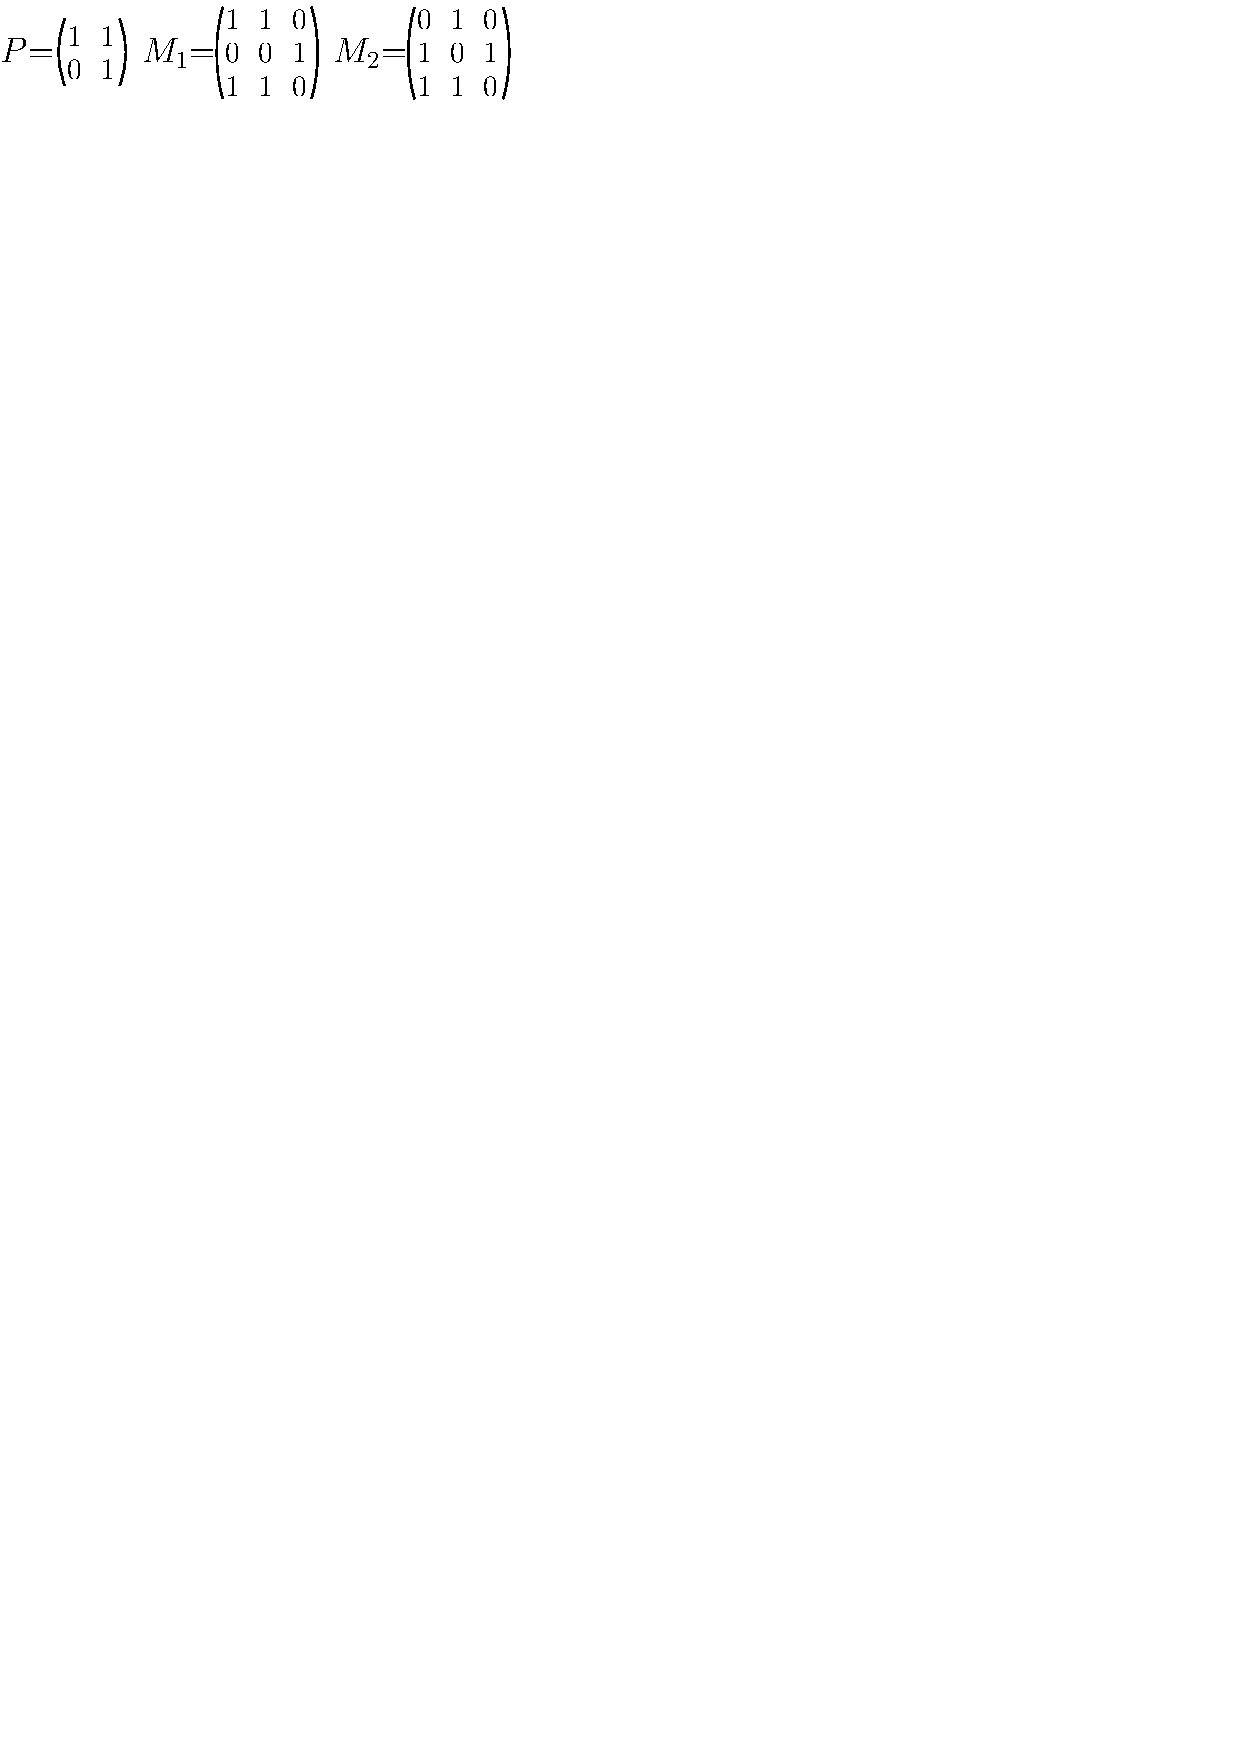
\includegraphics{../img/example.pdf}<1>
% Nejlépe je to vidět na obrázku, kde matice M_1 obsahuje P, protože vynecháním prostředního řádku a posledního sloupce dostaneme podmatici, která má jedničky tam, kde je má vzor. Naopak matice M_2 vzor P neobsahuje.
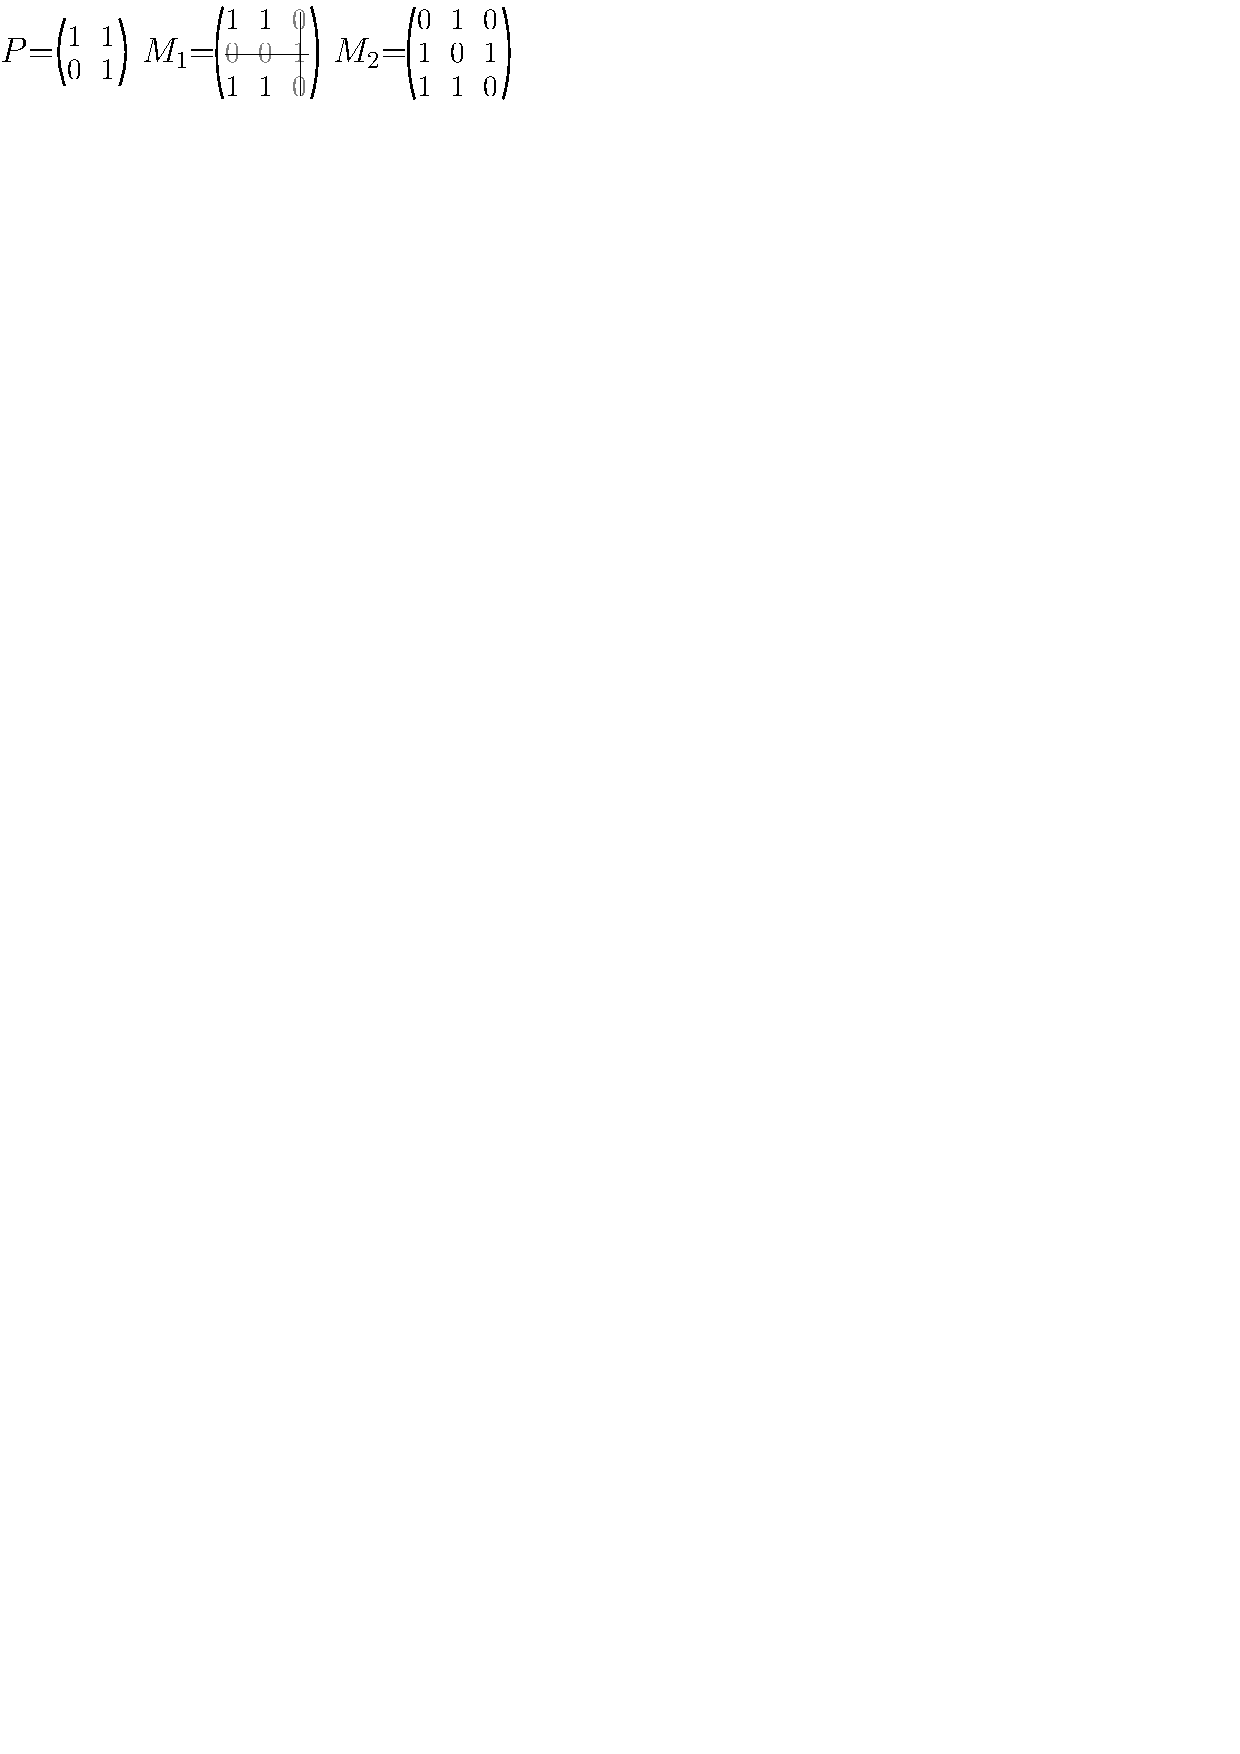
\includegraphics{../img/example2.pdf}<2>
\end{frame}

\subsection{Příklady použití}
\begin{frame}
\frametitle{Příklady použití}
\begin{itemize}
\setlength\itemsep{3mm}
\item Za pomoci matic bez~zakázaných vzorů se~dokázal horní odhad časové složitosti algoritmu Efrata a~Sharira na~``Segment-center problem''.
\item Existuje korelace mezi některými třídami matic bez~zakázených vzorů a~Davenport-Schinzelovým posloupnostmi, které souvisí se~složitostí dolní (horní) obálky arrangementů v~rovině.
%. Nejspíš jen přečtu, případně vysvětlím, kdyby se někdo zeptal.
% Teď, když vidíme, že může být zajímavé zkoumat třídy matic, které neobsahují zakázaný vzor, co může být pro testování hypotéz užitečnější, než si umět vygenerovat matici z libovolné třídy, která je náhodná.
\end{itemize}
\end{frame}

\section{Generování matic}
\subsection{Teoretické pozadí}
\begin{frame}
\frametitle{Markovovy řetězce}
\begin{block}{Definice (neformální)}
Pro předepsané pravděpodobnosti $p_{i,j}$ je \alert{Markovův řetězec} posloupnost $X_0,X_1,\dots$ prvků ze~stavové množiny $\mathcal{X}$ dodržující $P[X_{t+1}=j|X_t=i]=p_{i,j}.$
\end{block}
% K tomu použijeme teorii Markovoých řetězců a náhodných procesů nad nimi.
%. Přečtu.
% Následuje klíčová věta, na které stojí můj celý program.
\pause
\begin{block}{Věta (neformální)}
Pokud je Markovův řetězec aperiodický, nerozložitelný a~symetrický, potom je jeho limita uniformně náhodně rozložena na stavové množině $\mathcal{X}$.
\end{block}
%. Přečtu.
% Mým cílem je tedy navrhnout Markovův řetězec s témito vlastnostmi.
\end{frame}

\begin{frame}
\frametitle{Markovův řetězec pro matice}
Pokud chceme generovat matici neobsahující vzor $P$, postupujeme takto:
\begin{enumerate}
\item Zvolíme libovolnou matici $M$ neobahující $P$.
\item Změníme uniformně náhodně vybraný bit $M$, čímž dostaneme $M'$.
\item \alert<3>{Pokud $M'$ neobsahuje $P$ jako podmatici}, nastavíme $M:=M'$.
\item Goto 2.
\end{enumerate}
%. Přečtu svými slovy.
% 2. Uniformně náhodně vybereme řádek a sloupeček matice a příslušný bit změníme.
% 3. Pokud ... potom M' bude nové M.
% 4. Kroky 2 a 3 tvoří jednu iteraci procesu a my ho budeme opakovat mnohokrát.
\vspace{1em}
\onslide<2,3>
Protože definovaný Markovův řetězec splňuje předpoklady věty z~minulého slidu, je jeho limita náhodná matice neobsahující vzor $P$ jako podmatici. Bohužel zmíněná věta ani~žádná jiná (pro obecné Markovovy řetězce) nedává odhad na~dostačující počet iterací (mixing time), proto volbu počtu iterací necháme na~uživateli.
%. Přečtu.
% Zvýrazněná podmínka je tou algoritmicky nejsložitější a zbytek prezentace až na výjimky bude věnován jí. Nyní si ukážeme jak ji testovat pro matice, které mají speciální tvar.
\end{frame}

\subsection{Algoritmus pro testování speciálních vzorů}
\begin{frame}
\frametitle{Algoritmus pro testování speciálních vzorů}
\begin{block}{Definice}
O~matici řekneme, že je to \alert{Walking pattern}, pokud existuje procházka z~levého horního rohu matice do~pravého dolního rohu obsahující všechny jedničky v~matici.
\end{block}
%. Přečtu.
\vspace{5mm}
\centering
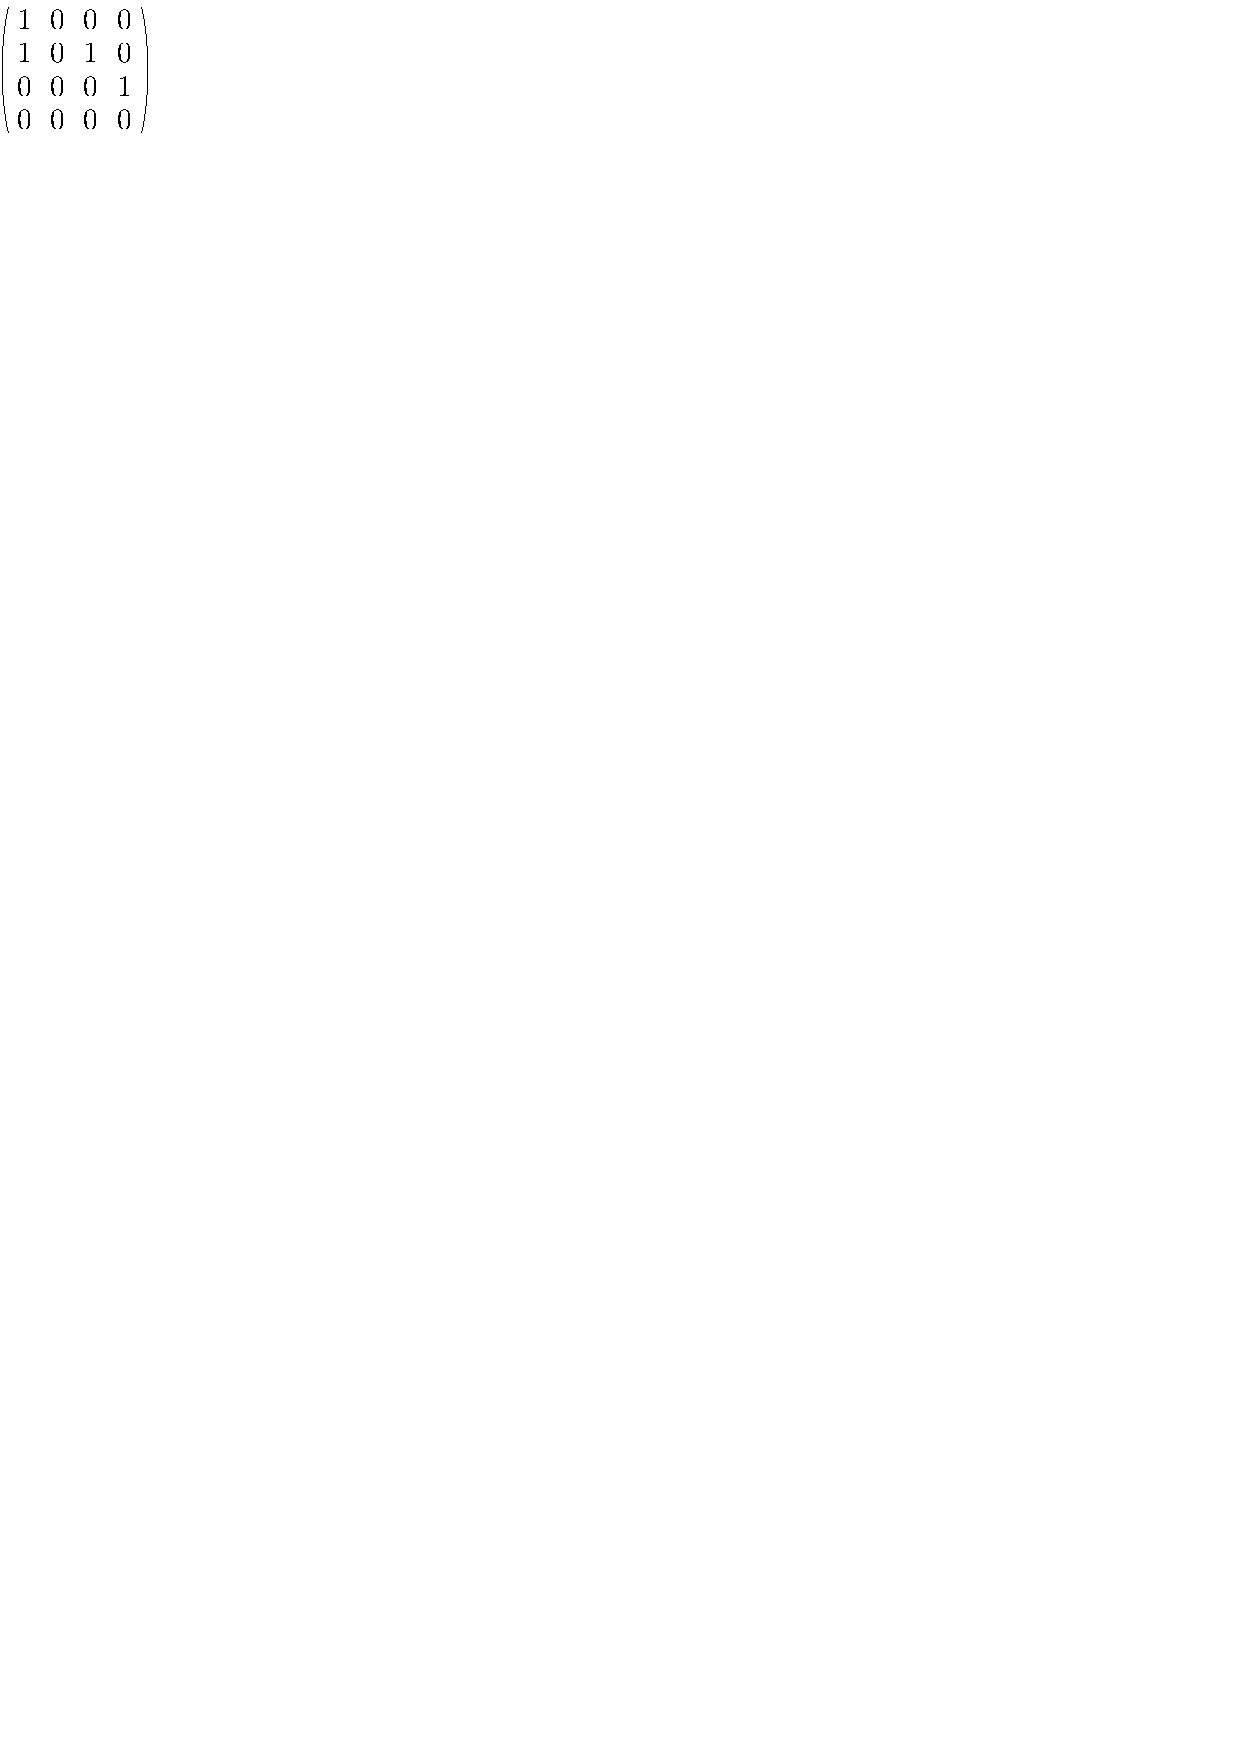
\includegraphics{../img/walkingexample1.pdf}<1>
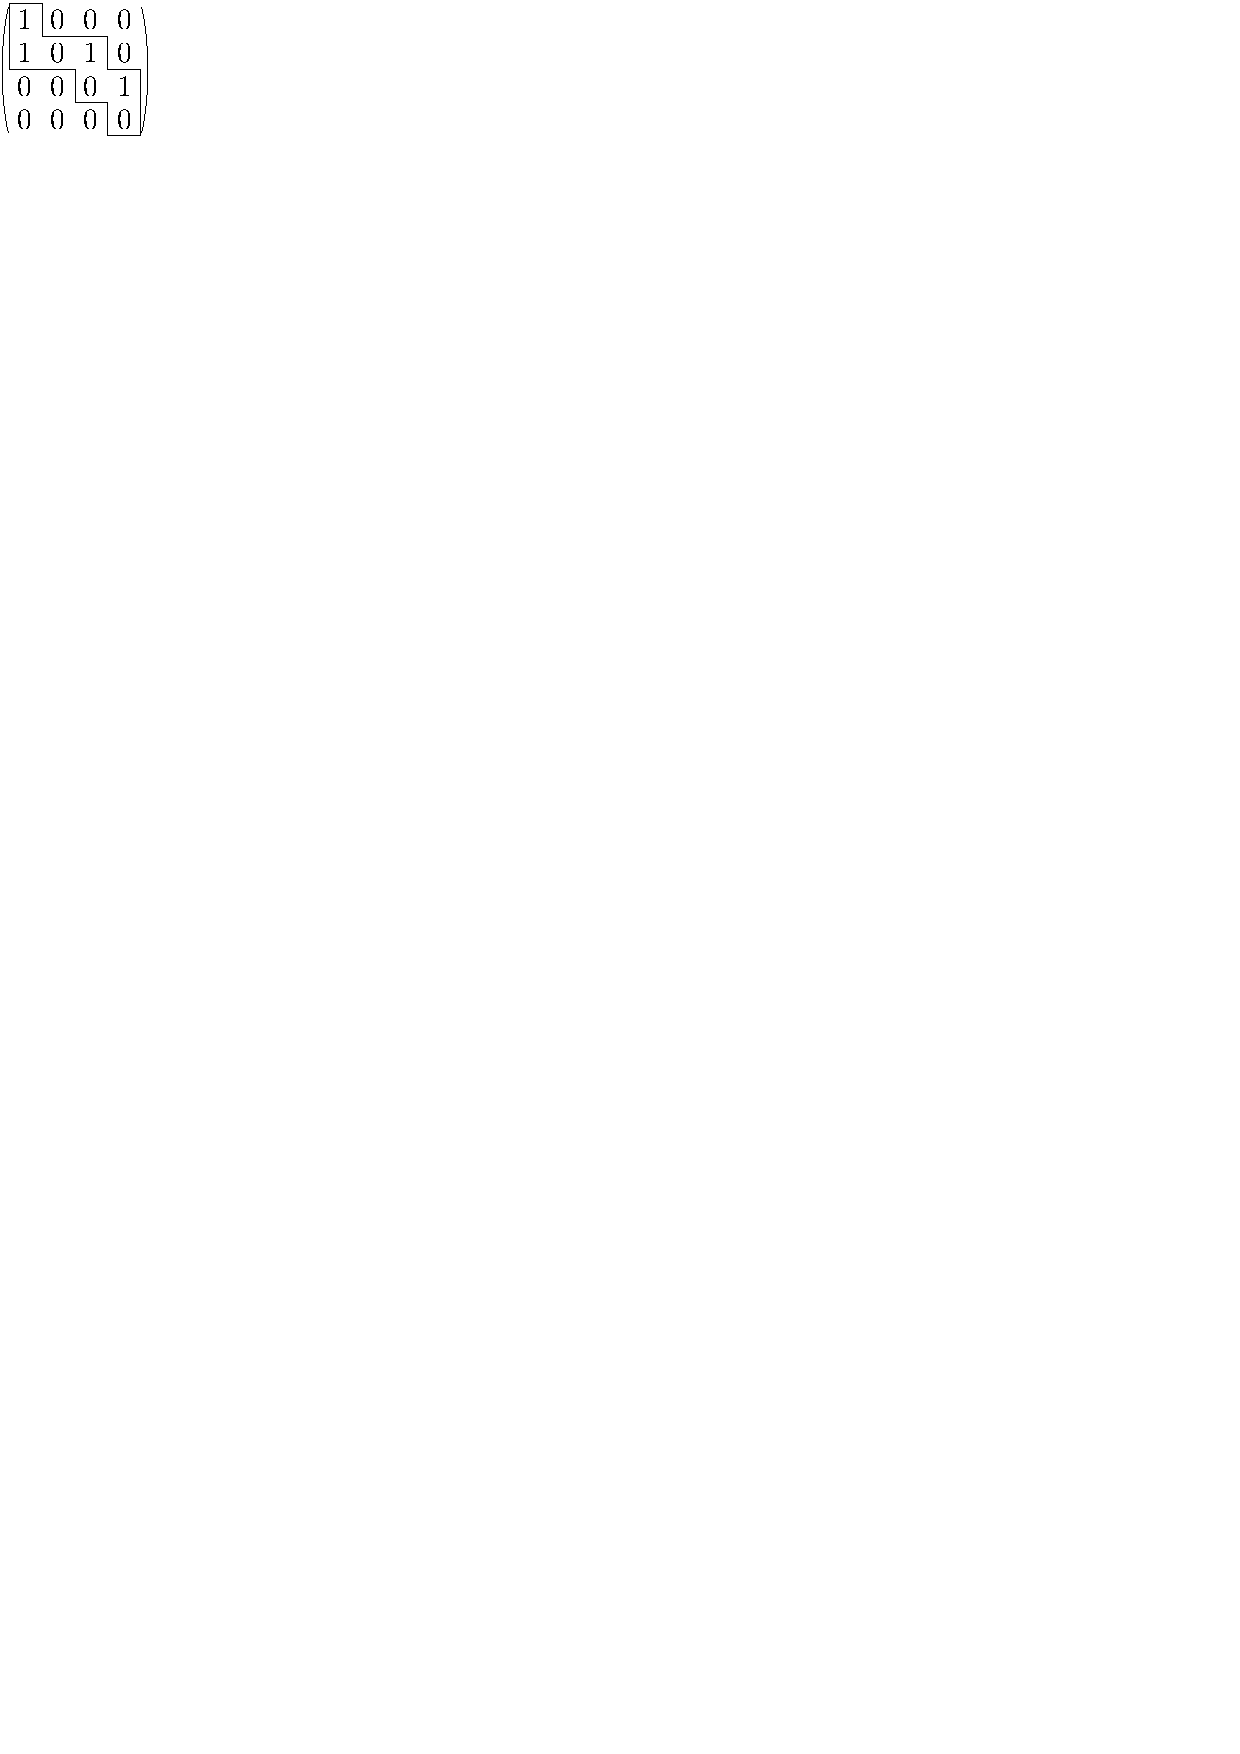
\includegraphics{../img/walkingexample2.pdf}<2>
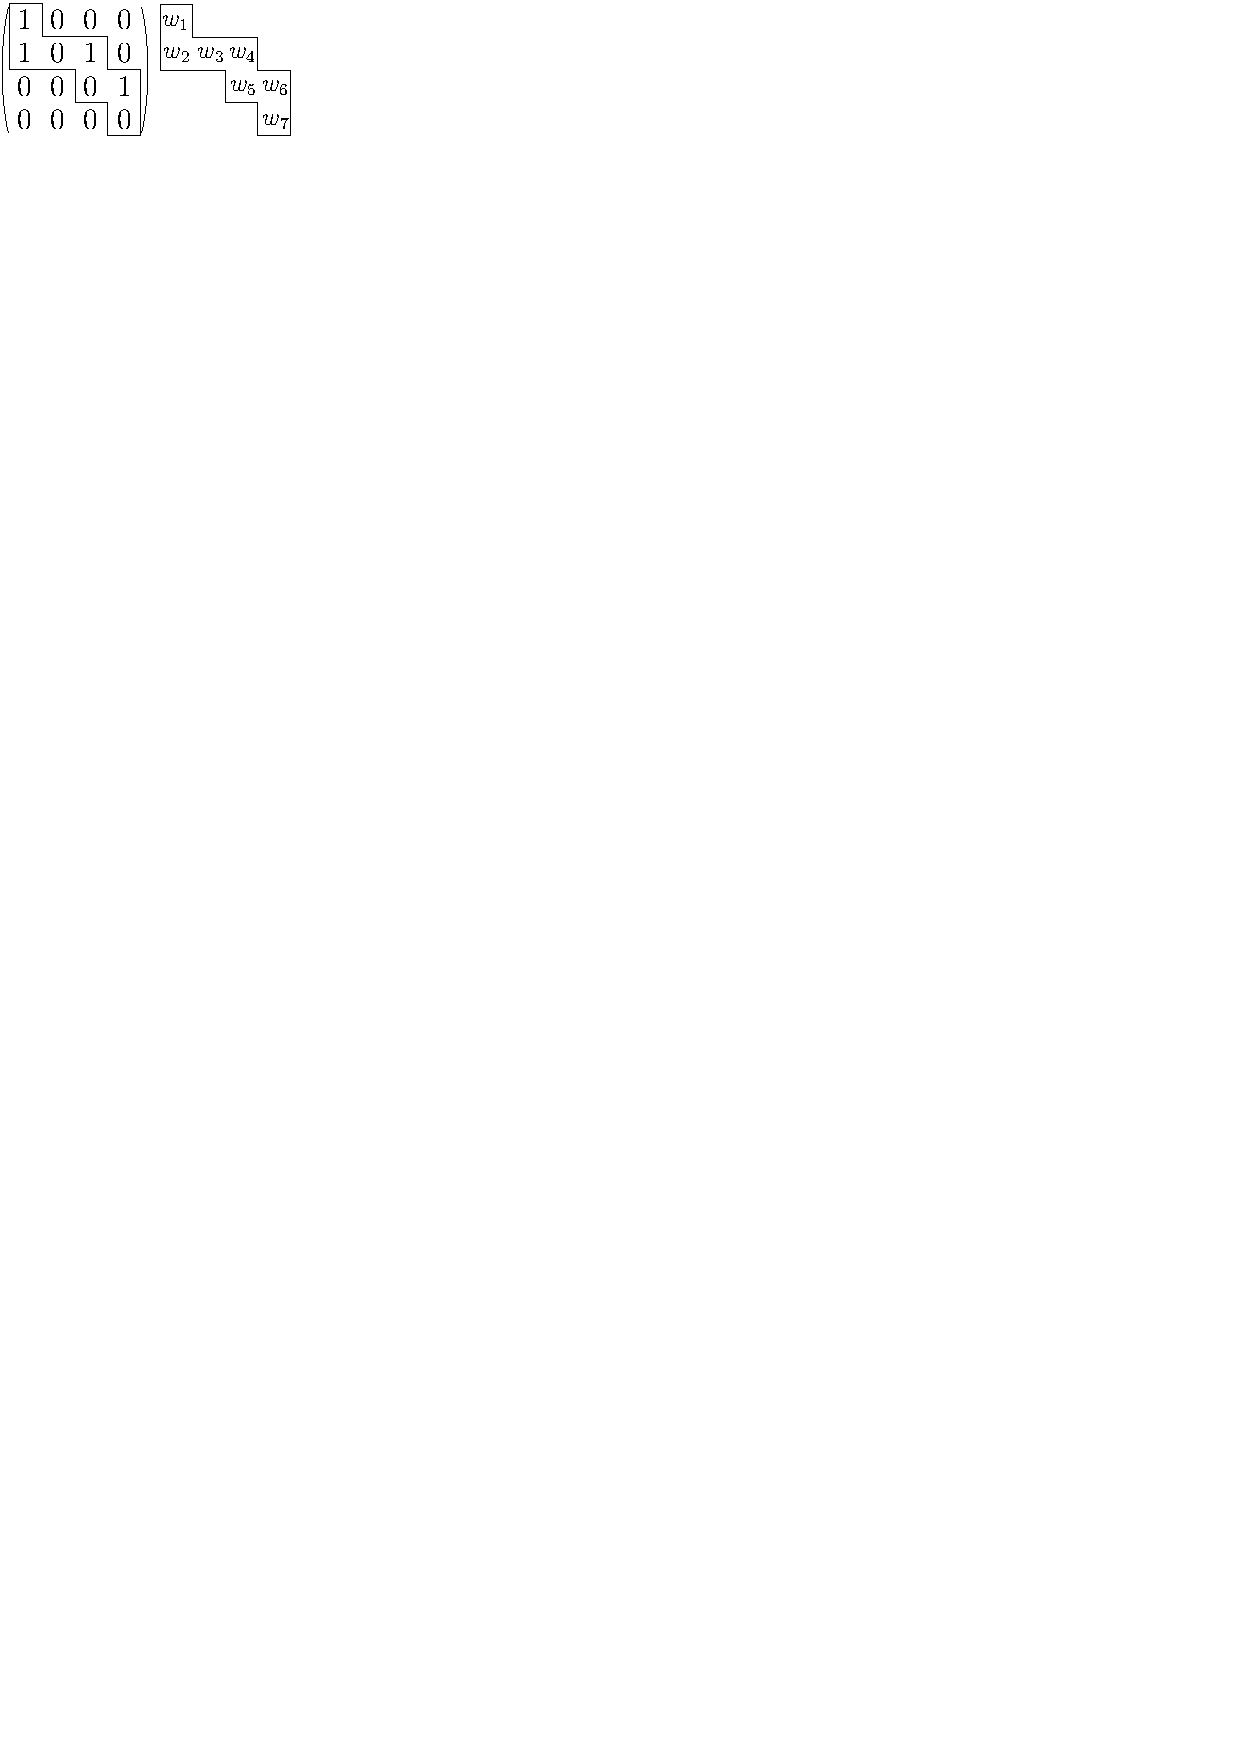
\includegraphics{../img/walkingexample3.pdf}<3>
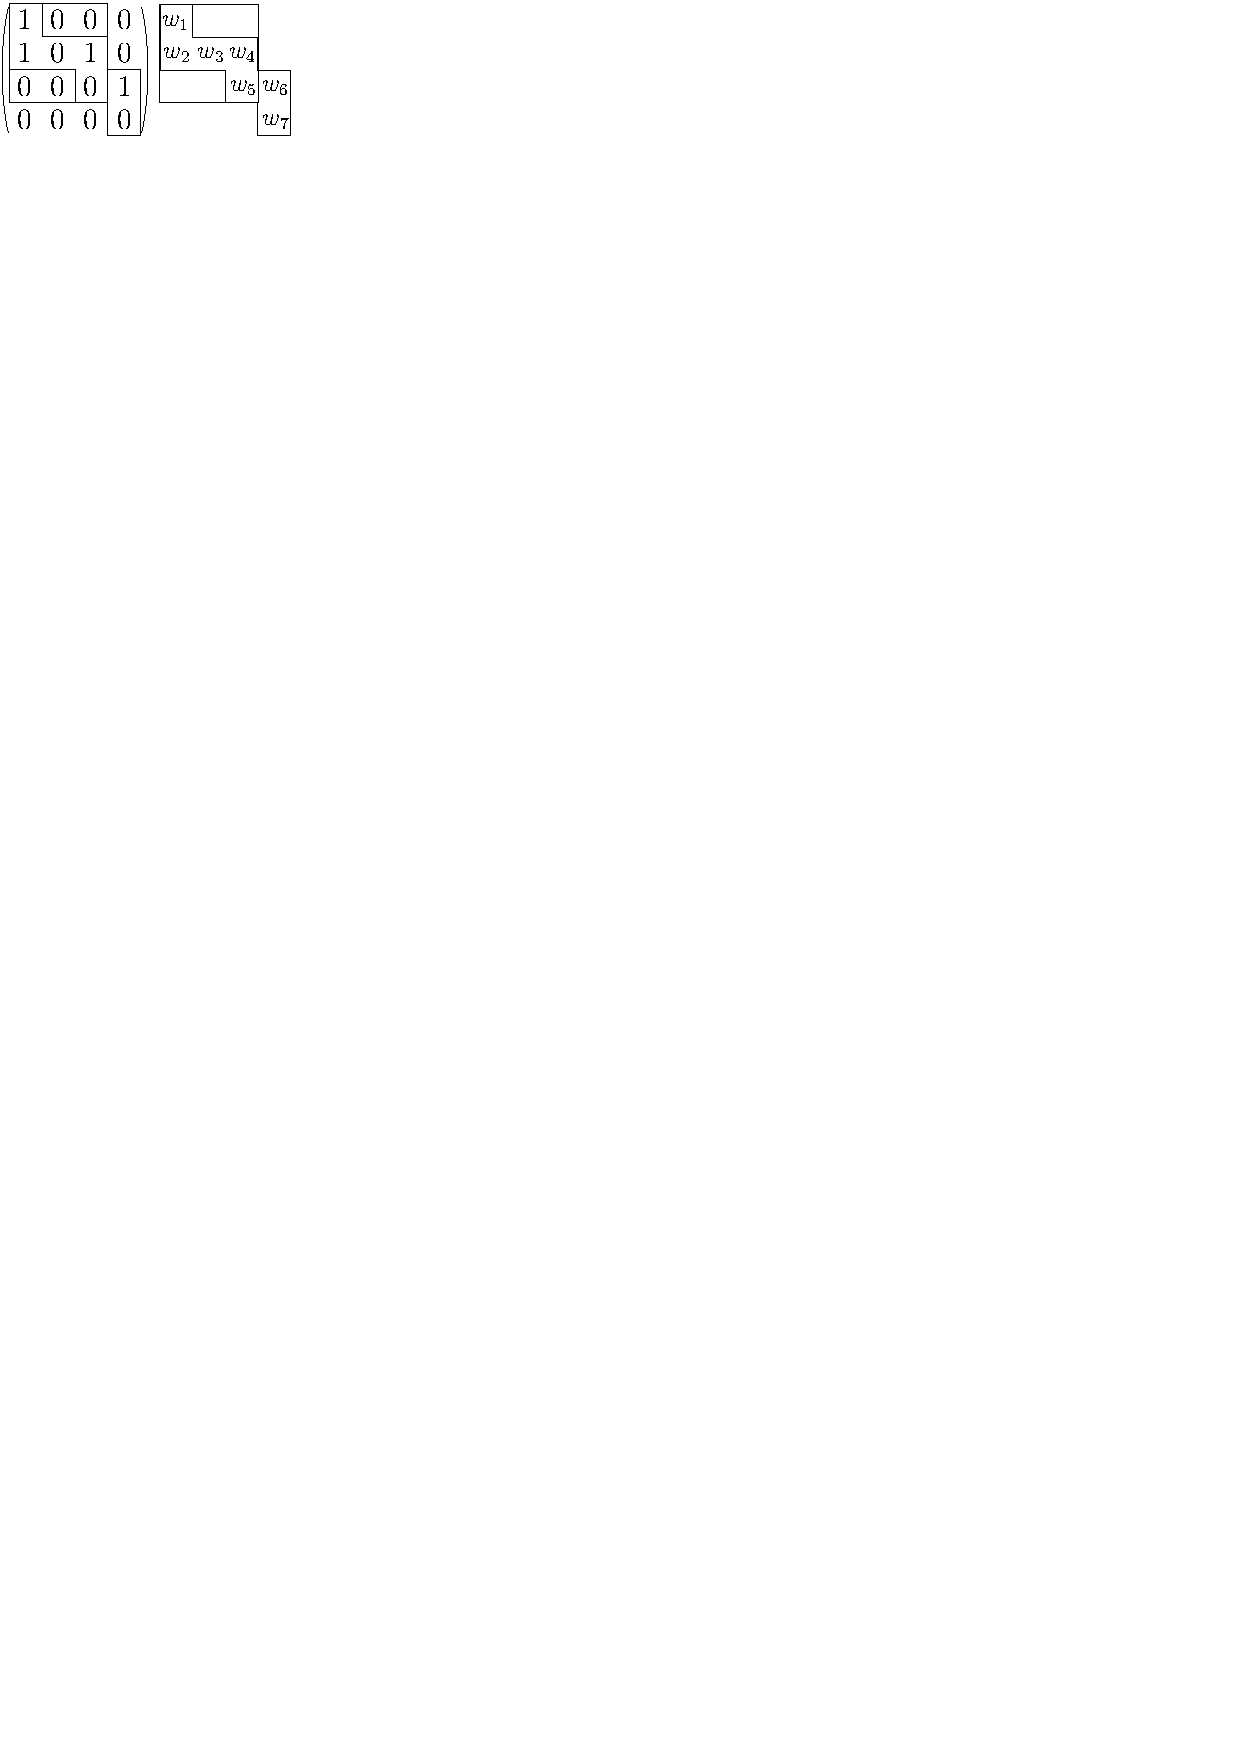
\includegraphics{../img/walkingexample4.pdf}<4>
% Na obrázku máme jeden takový vzor. Ona procházka je vyznačena v rámečku a všechny prvky procházky se ještě naznačeným způsobem oindexujeme. Když mluvíme o části vzoru až po 5-tý prvek, myslíme tím po 5-tý prvek procházky a máme tím na mysli vyznačenou podmatici vzoru.
\end{frame}

\begin{frame}
\frametitle{Algoritmus pro testování Walking pattern}
\centering
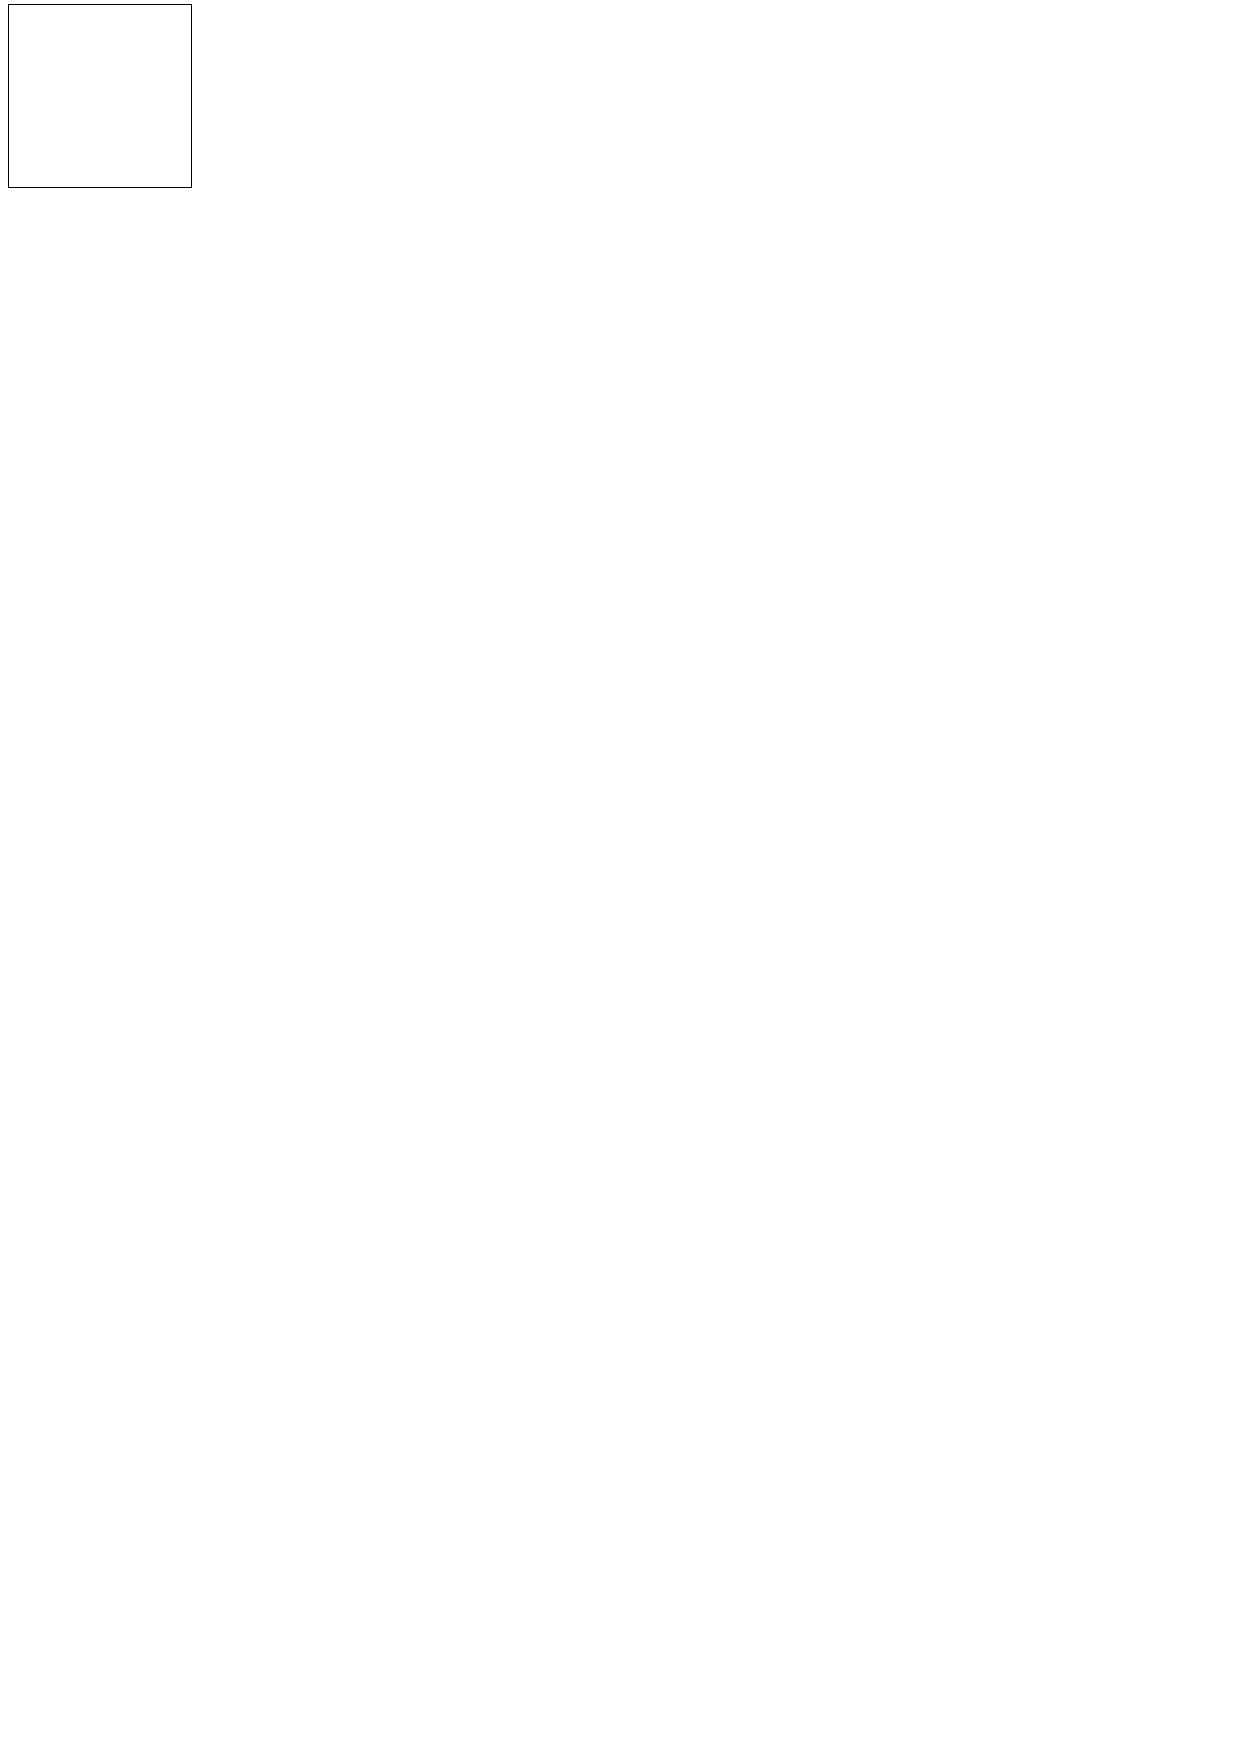
\includegraphics[scale=1.5]{../img/walkingalg0.pdf}<1>
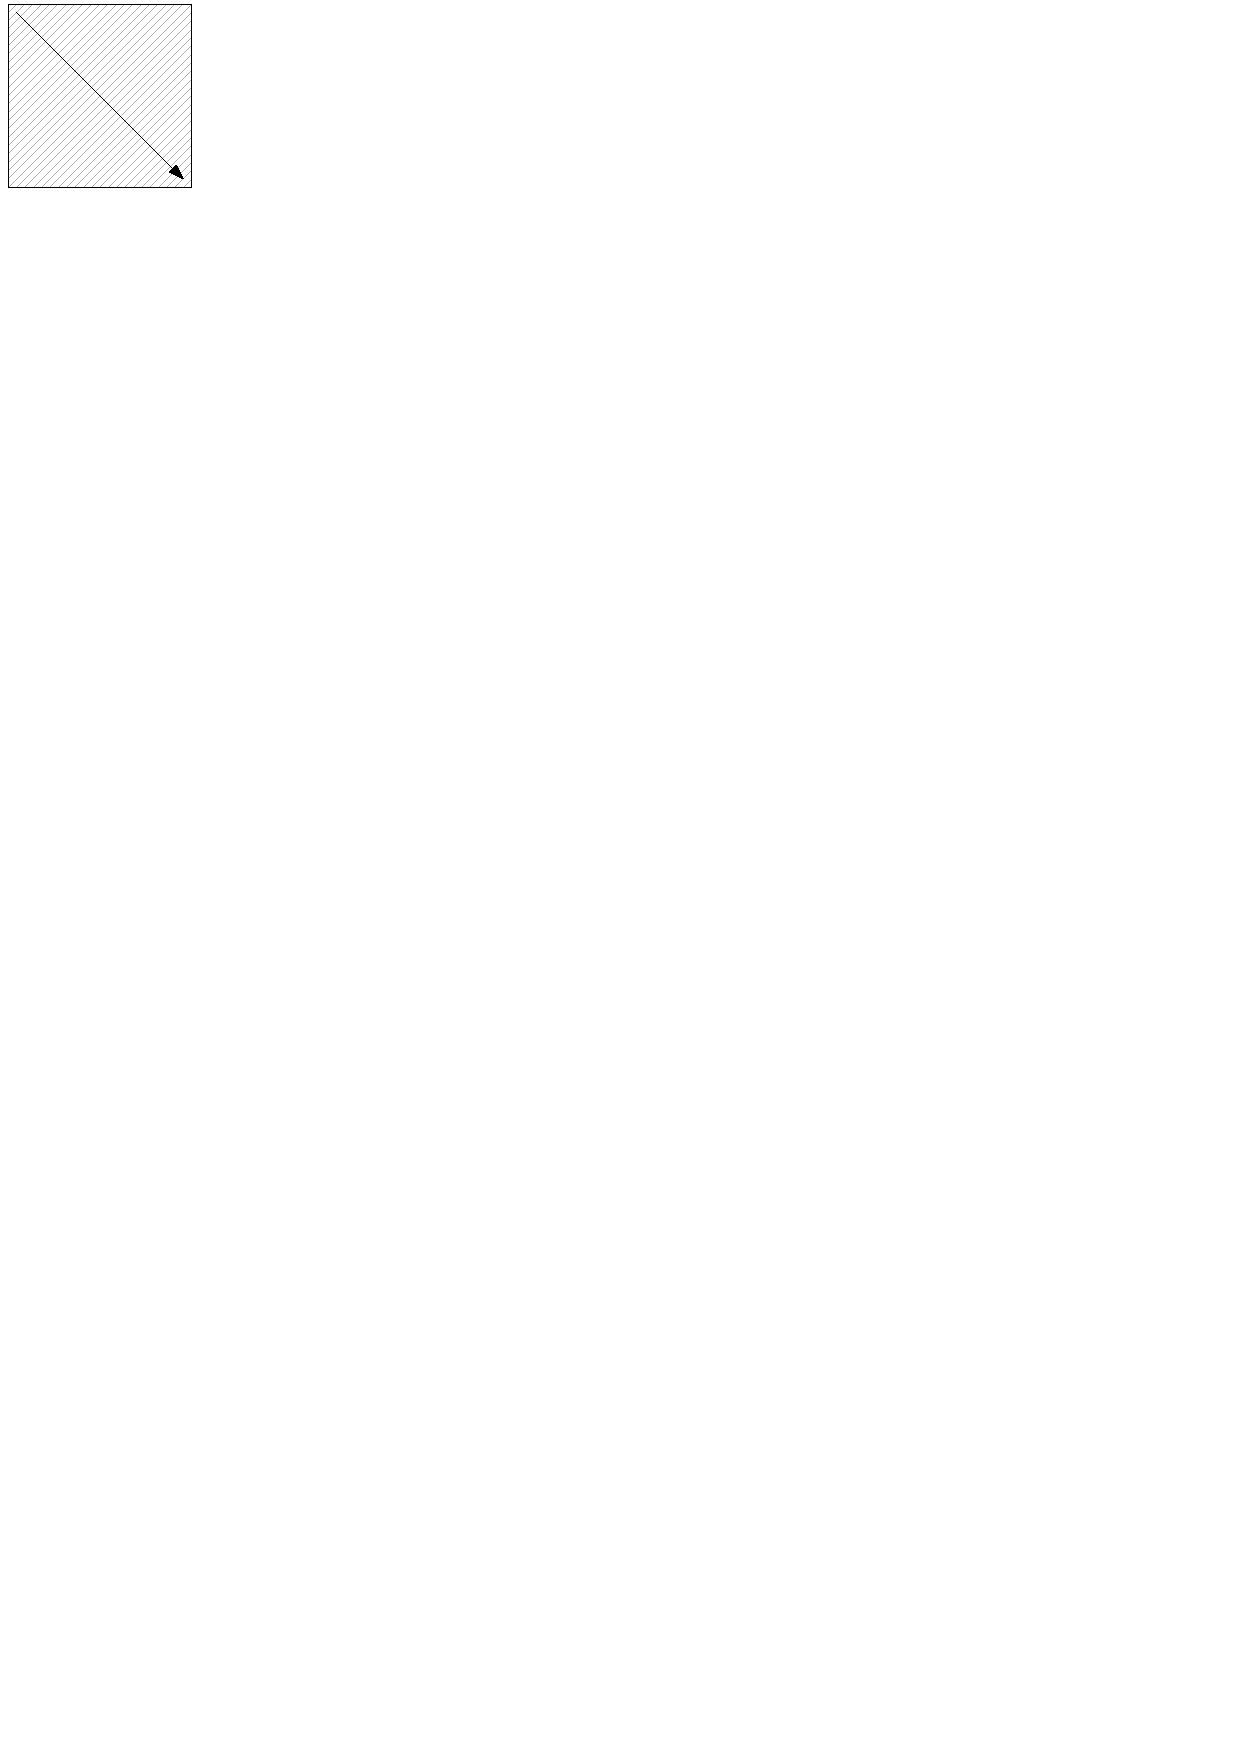
\includegraphics[scale=1.5]{../img/walkingalg1.pdf}<2>
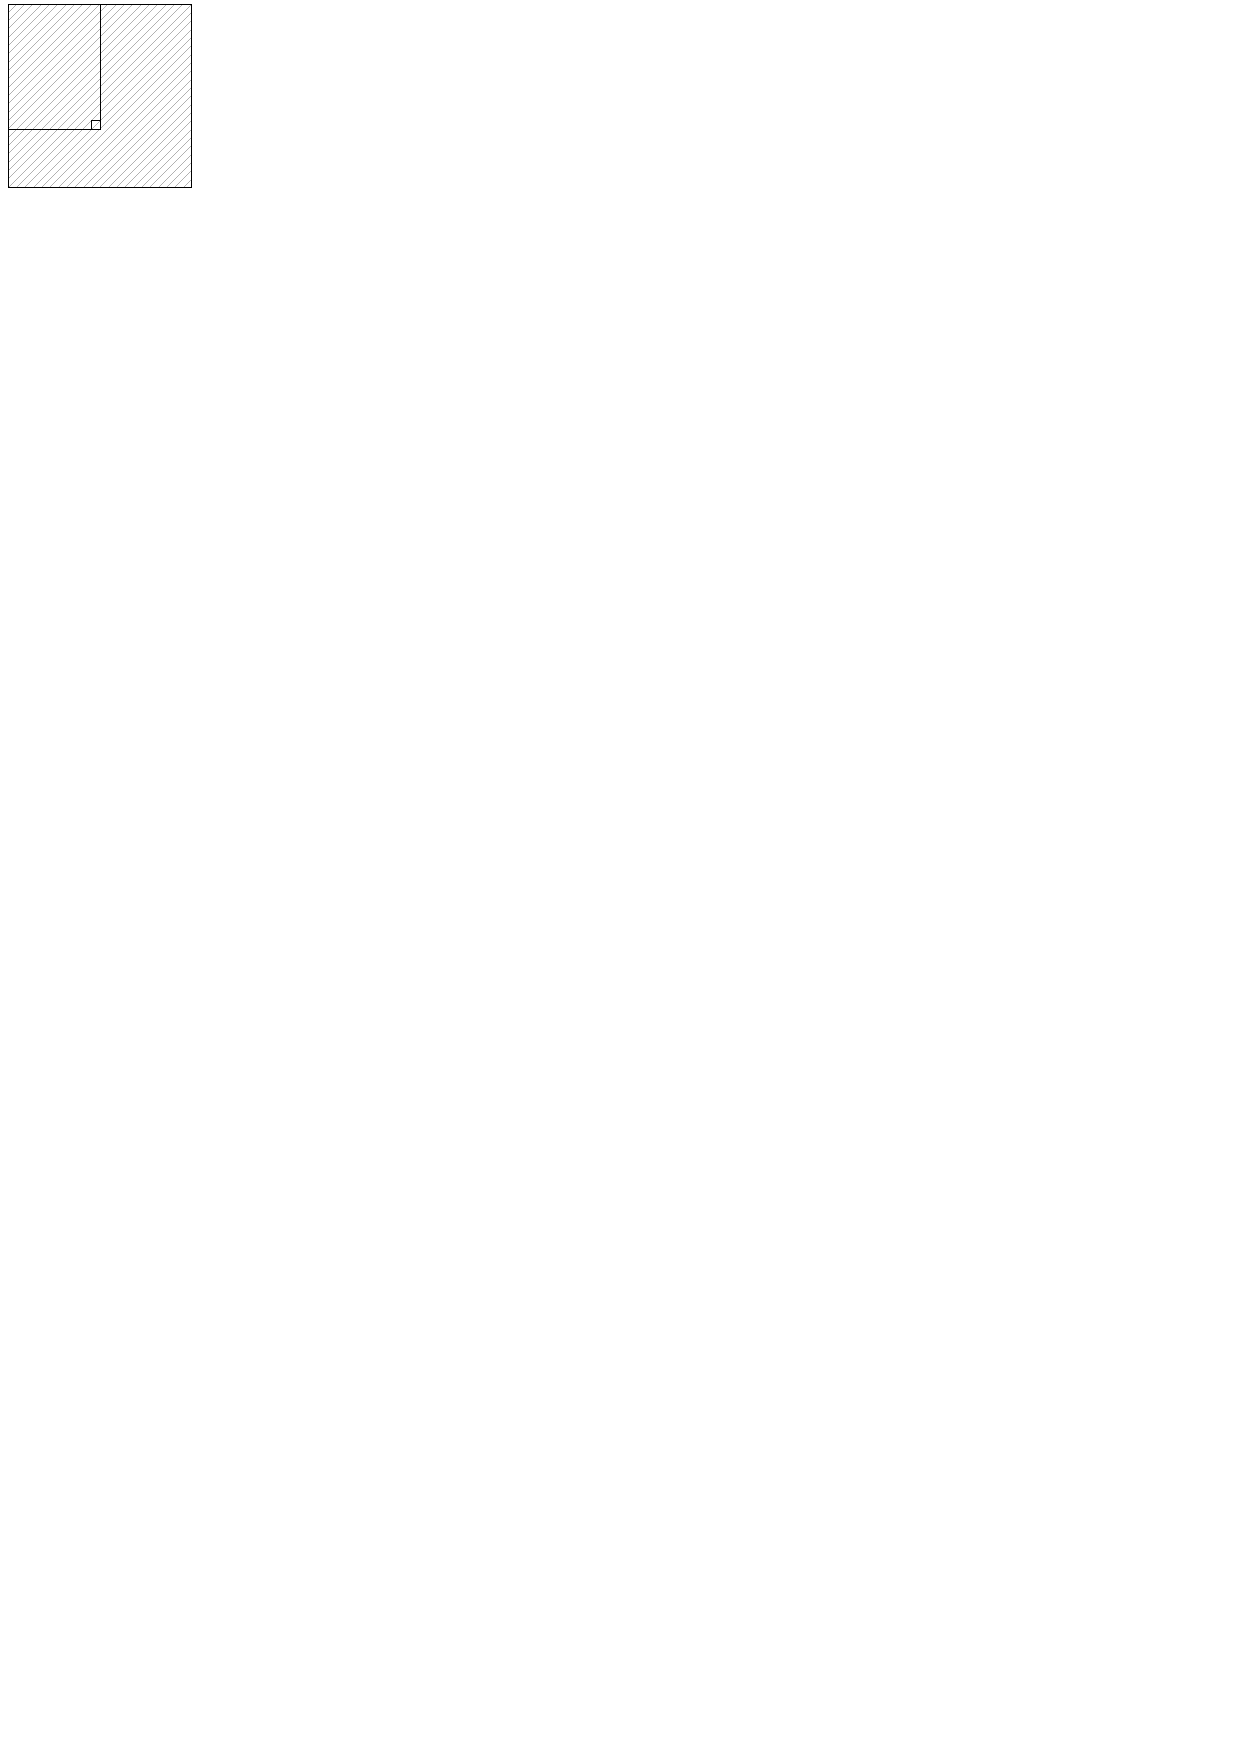
\includegraphics[scale=1.5]{../img/walkingalg2.pdf}<3>
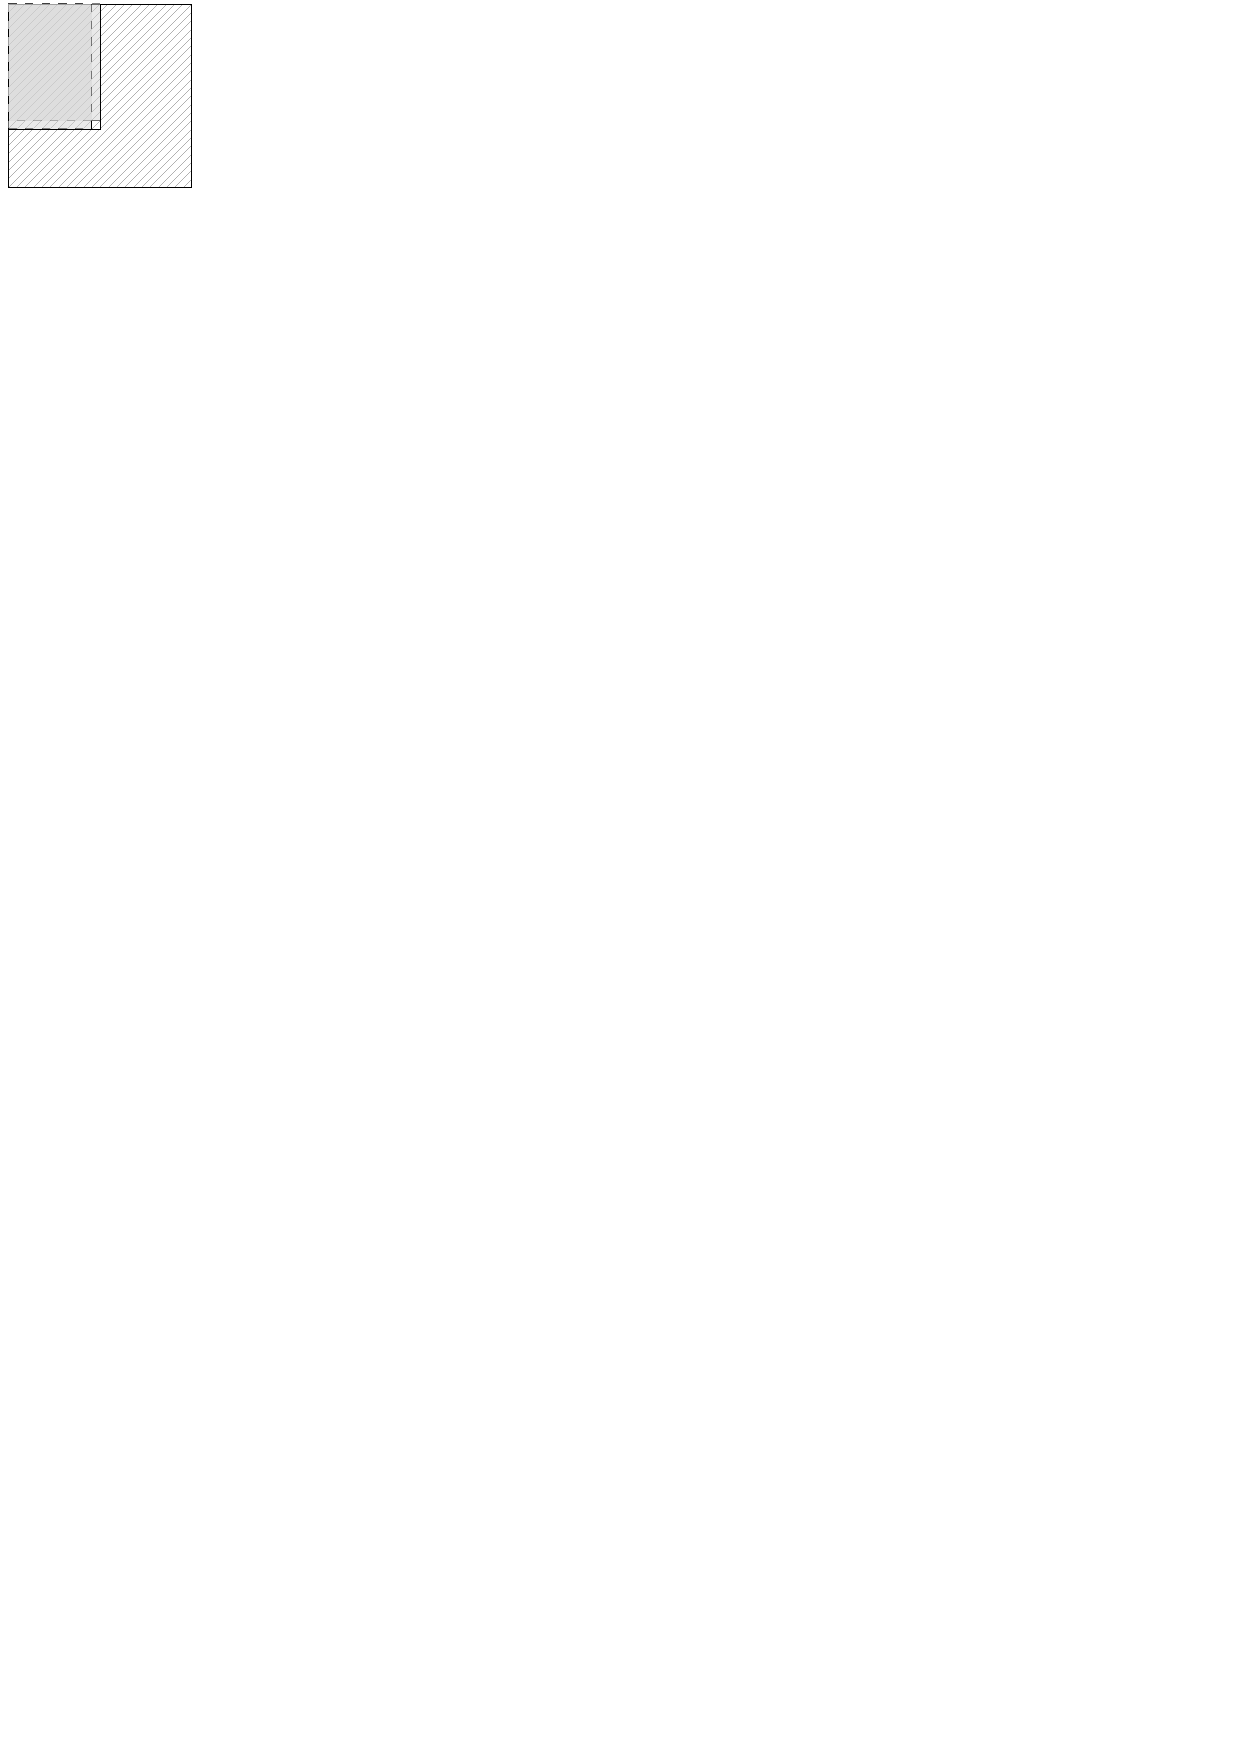
\includegraphics[scale=1.5]{../img/walkingalg3.pdf}<4>
% Mějme matici, pro kterou testujeme, zda obsahuje walking_pattern. Budeme postupovat po naznačených diagonálách ve směru šipky a pro každý prvek budeme chtít spočítat, jaká nejdelší část vzoru se vejde do podmatice určené tímto prvkem. Z hodnot spočítaných pro šedé podmatice už dokážeme v konstatním čase spočítat správnou hodnotu i pro počítaný prvek. Když během výpočtu narazíme na podmatici, do které lze namapovat i poslední prvek vzoru, pak je vzor obsažen a v opačném případě obsažen není.
% Dosáhli jsme tedy složitosti lineární s velikostí matice. Když si budeme pamatovat spočítané hodnoty i mezi iteracemi, můžeme iteraci ještě zrychlit, protože nebudeme přepočítávat celou matici, ale jen její změněnou část.
% Teď se podívejme na pomalejší algoritmus, který ale funguje pro všechny vzory.
\end{frame}

\subsection{Algoritmus pro testování obecných vzorů}
\begin{frame}
\frametitle{Algoritmus pro testování obecných vzorů}
Rozhodnout, zda daná matice obsahuje daný vzor je NP-úplné (dokonce
i~pro~permutační matice).\\
%. Přečtu.
% Proto použijeme brute-force algoritmus, ve kterém ...
\pause
\vspace{1em}
Při testování obsahování vzoru postupně mapujeme všechny linie (řádky a~sloupce) vzoru na~všechny možné linie testované matice.\\
%. Přečtu.
% Řádky samozřejmě mapujeme na řádky a sloupce na sloupce, navíc zachováváme pořadí linií. Ve svém programu se samozřejmě snažím tento brute-force algoritmus mnoha způsoby optimalizovat. Tady je seznam několika důležitých optimalizací.
\pause
\vspace{1em}
Optimalizace:
%. Bod vždy přečtu a pak k němu něco dodám.
\begin{itemize}
\item Některá částečná mapování můžeme sloučit a~tím ušetřit čas~i prostor.
% To, která mapování můžeme sloučit přímo závisí na volbě pořadí linií, ve kterém se budou mapovat, protože slučovat můžeme pouze ta mapování, která se liší pouze v namapování těch linií, které už jsou ze všech směrů omezeny. Tím myslím, že je namapována předchodchozí a následující linie, a také linie, které ji protínají v jedničce.
\pause
\item Program poskytuje mnoho různých způsobů jak zvolit pořadí, ve~kterém se budou linie mapovat.
% Ač se to tak nemusí na první pohled jevit, volba pořadí je zásadní pro rychlost testování a to hlavně kvůli předchozímu bodu. Efektivita různých voleb se liší vzor od vzoru a uživatel si pořadí může zvolit.
\pause
\item Volitelně program při mapování linie testuje, jestli je dost jedniček tam, kam se budou později mapovat dosud nenamapované linie.
\pause
% Tento popis obsahuje několikero různých heuristik, které může uživatel podle uvážení zapnout nebo vypnout a jejichž důsledkem je, že sice mapování jedné linie trvá déle, ale zase daleko rychleji poznáme, že vytvořené částečné mapování již nepůjde rozšířit na mapování celého vzoru.
\item Protože známe generující proces a již víme, že matice před změnou bitu vzor neobsahovala, víme také, že pokud ho po~změně obsahuje, tak jedině proto, že právě změněný bit je součástí mapování vzoru.
% Což znovu značně zmenšuje počet částečných mapování, které v průběhu program vytvoří.
\end{itemize}
\end{frame}

\begin{frame}
\begin{table}[]
\centering
\begin{tabular}{|ccc|c|r|c|c|c|c|r|}
\hline
\multicolumn{3}{|c|}{\textbf{Vzor}} & \textbf{n} & \textbf{\#iterací} & \textbf{pořadí} & \textbf{one} & \textbf{rek} & \textbf{ort} & \textbf{čas (s)} \\ \hline
 &  &  & 100 & 100 000 & MAX & ano & ano & ano & 121,85 \\ \cline{4-10}
 &  &  & 100 & 100 000 & MAX & ano & ano & ne & 120,80 \\ \cline{4-10} 
 &  &  & 100 & 100 000 & MAX & ne & ne & ne & 263,71 \\ \cline{4-10}
 &  &  & 500 & 10 000 & MAX & ano & ano & ano & 1 053,18 \\ \cline{4-10} 
1 & 0 & 0 & 500 & 10 000 & MAX & ano & ano & ne & 1 051,97 \\ \cline{4-10}
1 & 1 & 1 & 500 & 10 000 & \alert<1>{MAX} & ne & ne & ne & \alert<1>{2 695,26} \\ \cline{4-10} 
0 & 0 & 1 & 100 & 100 000 & DESC & \alert<3>{ano} & \alert<3>{ano} & \alert<3>{ano} & \alert<3>{82,39} \\ \cline{4-10} 
 & & & 100 & 100 000 & DESC & \alert<3>{ano} & \alert<3>{ano} & \alert<3>{ne} & \alert<3>{92,72} \\ \cline{4-10} 
 &  &  & 100 & 100 000 & DESC & \alert<3>{ne} & \alert<3>{ne} & \alert<3>{ne} & \alert<3>{113,34} \\ \cline{4-10} 
 &  &  & 500 & 10 000 & DESC & \alert<2>{ano} & \alert<2>{ano} & \alert<2>{ano} & \alert<2>{430,01} \\ \cline{4-10} 
 &  &  & 500 & 10 000 & DESC & \alert<2>{ano} & \alert<2>{ano} & \alert<2>{ne} & \alert<2>{446,21} \\ \cline{4-10} 
 &  &  & 500 & 10 000 & \alert<1>{DESC} & \alert<2>{ne} & \alert<2>{ne} & \alert<2>{ne} & \alert<1,2>{195,15} \\ \hline
\end{tabular}
\end{table}
% Efekt zmíněných vylepšení si ukážeme na této tabulce naměřených hodnot pro konkrétní vzor. Vše je spočítané se stejným seedem, což také znamená, že všechny odpovídající si výpočty vygenerovali stejnou matici. Červeně jsem označil 2 řádky, které se liší pouze ve volbě pořadí mapování řádků a sloupců, a vidíme, že rozdíl je obrovský. Tady ještě zmíním, že pro jiné vzory může být naopak první pořadí rychlejší než to druhé. Pak se zaměřme na zapnutí různých heuristik. Vidíme, že výpočet doběhne nejrychleji pokud žádnou z heuristik nepoužijeme. Naopak ale, když budeme generovat menší matici, nejlépe to dopadne, pokud použijeme všechny heuristiky.
\end{frame}

\subsection{Paralelní počítání}
\begin{frame}
\frametitle{Vícevláknové generování}
Pokud generujeme dostatečně velkou matici a už je dostatečně zahuštěná, potom pravděpodobnost, že nějaká změna bitu uspěje, je malá, a tedy většina iterací neuspěje (matice zůstane taková, jaká byla před iterací).\\
\vspace{1em}
\onslide<2,3> Idea: pro generovanou matici $M$ si místo jedné vybere $p$ pozic, pro~každou samostatně změníme určených bit $M$, čímž dostaneme $p$ matic $M'$. Pro~každou z~nich otestujeme obsahování vzoru, a podle výsledků vybereme, které změny na~matici $M$ provedeme.\\
% místo abychom provedli jen jednu jednobitovou změnu v generované matici a testovali obsahování vzoru, provedeme jednobitových změn několik (paralelně) a výsledek získáme \alert<3>{výběrem některých změn} ze všech provedených (některé výpočty tedy poběží aniž by měly vliv na generovanou matici).\\
\vspace{1em}
\onslide<3> Výběr změn, které ovlivní generovanou matici musíme dělat opatrně, aby stále neobsahovala zakázaný vzor, a zároveň se proces držel definovaného Markovova řetězce, a tedy konvergoval k náhodné matici.
% Program si poradí i s více vlákny. Využívá při tom toho, že ...
% ... uspěje, tedy M' neobsahuje P jako podmatici.
% Přesnější vysvětlení by zabralo příliš mnoho času, proto ho vynechám. Zmíním jen to, že součástí implementace je optimalize v podobě spekulativního počítání, kdy považujeme nějakou změnu bitu za provedenou i ve chvíli, kdy ještě nevíme, že tuto změnu smíme provést.
\end{frame}

%\begin{frame}
%\frametitle{Vícevláknové generování}
%Výběr změn, které ovlivní generovanou matici musíme dělat opatrně, aby stále neobsahovala zakázaný vzor a zároveň se proces držel definovaného Markovova řetězce a tedy konvergoval k náhodné matici.\\
%\pause
%\vspace{1em}
%Za tímto účelem si udržujeme pořadí, ve kterém se jednotlivé výpočty obsahování spustili, a potom čekáme na skončení toho výpočtu, který je v tomto pořadí první ze všech dosud nezpracovaných. Pokud tento výpočet neuspěje, započítáme neúspěšnou iteraci a jdeme dál. Pokud výpočet uspěje, znamená to, že všechny ostatní nezpracované výpočty počítali zbytečně, protože generovaná matice se touto iterací změnila.\\
%\pause
%\vspace{1em}
%Tohle přináší neefektivitu v případě, že výpočet, na který čekáme trvá dlouho. Pak se snadno stane, že ostatní nezpracované výpočty už doběhly a jen čekají, než na ně přijde řada. Jako řešení zavádíme spekulativní počítání, které zpracovává i výpočty, které zatím nejsou na řadě (ikdyž zatím nemůžou ovlivnit generovanou matici, protože stále může uspět výpočet v pořadí před nimi) a vláknu, které by jinak jen čekalo zadáme nový výpočet. 
%%. Už jen přečíst tohle zabere spoustu času.
%\end{frame}

\begin{frame}
\begin{table}[]
\centering
\begin{tabular}{|ccc|c|r|c|c|r|}
\hline
\multicolumn{3}{|c|}{\textbf{Vzor}} & \textbf{n} & \textbf{\#iterací} & \textbf{\#workerů} & \textbf{spekulace} & \textbf{čas (s)} \\ \hline
 &  &  & 100 & 100 000 & \alert<1>{1} & - & \alert<1>{82,39} \\ \cline{4-8} 
 & & & 100 & 100 000 & 4 & ano & 24,37 \\ \cline{4-8} 
 &  &  & 100 & 100 000 & 4 & ne & 26,68 \\ \cline{4-8} 
1 & 0 & 0 & 100 & 100 000 & \alert<1>{8} & ano & \alert<1>{14,74} \\ \cline{4-8}
1 & 1 & 1 & 100 & 100 000 & 8 & ne & 16,70 \\ \cline{4-8}
0 & 0 & 1 & 500 & 10 000 & \alert<2,3>{1} & - & \alert<2,3>{430,01} \\ \cline{4-8} 
 & & & 500 & 10 000 & 4 & ano & 152,11 \\ \cline{4-8} 
 &  &  & 500 & 10 000 & 4 & ne & 162,65 \\ \cline{4-8} 
 &  &  & 500 & 10 000 & \alert<2,3>{8} & \alert<3>{ano} & \alert<2,3>{92,10} \\ \cline{4-8}
 &  &  & 500 & 10 000 & \alert<3>{8} & \alert<3>{ne} & \alert<3>{121,26} \\ \hline
\end{tabular}
\end{table}
% Podívejme se ještě jednou na tabulku naměřených hodnot pro tento vzor. Na vyznačených řádcích vidíme, že když použijeme místo sériového výpočtu 8 workerů, kde počet workerů zhruba odpovídá počtu vláken, nedosáhneme sice 8x rychlejšího výpočtu, ale docela se tomu přiblížíme. Pro větší generovanou matici a menší počet iterací už zrychlení není tak markantní, ale zase je dobře vidět, že spekulativní výpočet přinesl své ovoce.
\end{frame}

%\begin{frame}
%\frametitle{Poděkování}
%\centering
%Děkuji svému vedoucímu za ochotu se vším mi pomoci a čas a úsilí, které mé práci věnoval.\\
%\vspace{1em}
%Děkuji svému oponentovi, že posudek odevzdal dříve než včas.\\
%\vspace{1em}
%Děkuji katedrám KAM a IÚUK za možnost pro své experimenty používat jejich výpočetní servery.
% Děkuji hlavně svému vedoucímu, že mi pomohl vytvořit program, na který můžu být hrdý.
%\end{frame}

\begin{frame}
\centering
Děkuji za pozornost.
\end{frame}

\begin{frame}
\frametitle{Pravděpodobnost úspěchu iterace}
Pokud se dívám na vzor, kde každá vygenerovaná matice velikosti $N\times N$ má nejvýš $cN$ jedniček, potom v~dlouhodobém průměru s~pravděpodobností nejvýš $cN/N^2=c/N$ program jedničku změní na~nulu, a~tedy v~průměru také s~pravděpodobností nejvýš $c/N$ program úspěšně změní nulu na~jedničku, protože počet jedniček bude zhruba konstantní. Pravděpodobnost neúspěšné změny by měla být aspoň $1-2c/N$, čímž podíl neúspěšných kroků poroste s~$N$.
\end{frame}

%. Citace přidávat nebudu.

%. Otazky oponenta:
%Q: Jedine, co mi chybelo, bylo v zaveru Kap. 4 podobnejsı rozbor pouzitych metod. Napr.: jaky je prınos spekulativnıch vypoctu (Sekce 4.2.2)? Jaky je optimalnı pocet vlaken? Jaky pocet iteracı je potreba pro dostatecne presnou aproximaci uniformnıho rozdelenı? (Zde by asi byla potreba kvantitativnı verze Vety 2.)
%A: Do prezentace jsem přidal tabulku s porovnáním paralelismu s a bez spekulace. Verzi bez spekulace jsem udelal ze soucasne verze projektu, takze je trochu pomalejsi nez by byt mohla, ale pro ilustraci to snad postaci. Optimalni pocet vlaken neznam. Program jsem zkousel pouze na kamenolomu (na kamenozroutu nikdy nebylo uplne volno a nikde jinde vice jader neni), a podle dat namerenych tam ani pro maximum (16) workeru vykon neklesa. Jaky je dostatecny pocet iteraci neumime my ani panove Liu s Madrasem vetou na zpusob Vety 2 zodpovedet. Madras a Liu zkoumali tuto velicinu experimentalne (precetl jsem si tu stranku, na ktere popisuji jak ziskavaji data, kde se vzalo 10^7 jsem z toho nevykoukal a prijde mi, ze neni duvod si myslet, ze stejne cislo bude fungovat u matic, ale minimalne sem muzu oponenta odkazat).

%Q: str. 8, Irreducibility: textu by odpovıdalo “we can always reach M1 from M2”
%A: Prohodil jsem M_1 a M_2.

%Q: str. 9/10: v definici important line by bylo vhodne vyjasnit, co znamena “adjacent line”. Dale: nemela by definice znıt: “at least on of the conditions is met”?
%A: Změnil jsem na: "The line~$l$ is the predecessor or successor of a line not in $(l_1,\dots,l_k)$", přidal "at least" a vlozil pagebreak pred definici.

%Q: str. 10: za nestastne povazuji znacit symbolem l dve ruzne veci (line a level).
%A: Změnil jsem druhé l na k, které už se ve stejném významu vyskytuje dříve.

%Q: a zejmena: bylo by asi vhodne nekde peclive vysvetlit, jak se unimportant lines a equivalent mappings pouzıvajı v implementaci.
%A: V 4.1.1 říkám, že v rámci paměťových úspor si mapování unimportant lines vůbec nepamatuji, čímž se ekvivalentní mapování v mém slova smyslu stávají totožnými mapováními ve smyslu C++.

%Q: str. 15: “fully bounded” znı divne, nemyslıte “fully restricted”?
%A: Změnil jsem "bounded" na "restricted".

%Q: str. 17–19: jednotlive heuristiky pro vyloucenı castecnych zobrazenı by stala za lepsı vysvetlenı. Zejmena Recursive mapping a Orthogonal bounds se mi spatne chapaly, a obrazek 4.4 je ponekud matoucı (co kupr. znacı dvojite sipky?).
%A: Tohle je něco, co se bude velmi špatně vysvětlovat u obhajoby. Obrázek je podle mě popsán dostatečně, jen tam chybí popis těch šipek, které mají znázorňovat, kde se hledá dostatečný počet jedniček. Ve slovních komentářích jsem pak hlavně spoléhal na obrázky, protože slovně se mi to popisuje velmi špatně. (Zatím jsem nijak neměnil, ikdyž bych asi měl)

%Q: str. 19, konec Sekce 4.1.5: bylo by hezke zmınit, pro ktere vzory zavisı ucinnost omezujıcıch heuristik na velikosti matice.
%A: Do prezentace přidána tabulka, kde je jeden takový vzor otestován. Těžko říci, pro jaké vzory tato závislost existuje. Můj odhad je, že pro všechny, ale nemám k tomu žádný pádný důvod.

%Q: str. 20: pro posouzenı ucinnosti MCMC paralelismu by bylo vhodne uvest, jaka je pravdepodobnost uspechu jedne iterace (treba experimentalne namereno, pokud nenı mozne teoreticky odvodit).
%A: Experimentálně naměřit si to s použitím mého programu a sériového výpočtu se zapnutím performance statistik může uživatel dokonce pro libovolný vzor. Je pravda, že tohle nikde není zmíněné, protože jsem performance statistiky používal hlavně pro svou potřebu, ale je to možné. Lepsi odpoved je v prvnim slidu za prezentaci. Jde o vytazek z emailu od meho vedouciho.

%Q: str. 21, predposlednı radka: narust o vıce nez jedna se asi neuskutecnı, pokud uspeje az poslednı z rady workeru, ne?
%A: To je pravda, muze se stat, ze se ID zvysi jen o jedna. Zmenil jsem "by more then one" na "by potentially more than one" a jeste jedno jine "then" na "than".

\end{document}